\documentclass[12pt]{article}

\usepackage{amsmath, amssymb, amsthm, graphicx, fancyhdr, textcomp, enumerate, diagbox, tcolorbox, esvect, tikz, adjustbox}


\graphicspath{{./images/}}


\usepackage{halloweenmath, tikzsymbols}

\newcommand{\R}{\mathbb{R}}
\newcommand{\Z}{\mathbb{Z}}
\newcommand{\C}{\mathbb{C}}
\newcommand{\N}{\mathbb{N}}
\newcommand{\Q}{\mathbb{Q}}
\newcommand{\Arg}{\mbox{Arg}}
\newcommand{\Log}{\mbox{Log}}


%geometry/topology
\newcommand{\bndry}{\partial}


\newcommand{\infsum}{\sum_{n = 1}^{\infty}}
\newcommand{\pf}{\fbox{proof}}
\newcommand{\cor}{\fbox{corollary}}

\theoremstyle{definition}

\newtheorem*{definition}{Definition}
\newtheorem{lemma}{Lemma}
\newtheorem{theorem}{Theorem}
\newtheorem{corollary}{Corollary}
\newtheorem{proposition}{Proposition}
\newtheorem{remark}{Remark}
\newtheorem{conjecture}{Conjecture}
\newtheorem{example}{Example}

\title{Modern Geometry}
\author{August}

\begin{document}

\maketitle

\begin{proposition}(1.5)

Given a polygon $P$, with a polygonal hole $H$ contained entirely within the interior of $P$, such that all of the vertices are in general position, the interior region can be triangulated. 
\end{proposition}

\begin{lemma}
Let $T$ be a triangle, and let $L$ be a line through points $p_1$ and $p_2$, which are in general position with respect to the vertices of $T$. Suppose that $L \cap T \ne \emptyset$. Then $L$ intersects two distinct edges of $T$. Moreover, the polygons formed by dividing $T$ through the line $L$ is convex. Also, both of these regions contain at least one of the vertices of $T$, and they do not share any of the vertices of $T$.
\end{lemma}

\begin{proof}
Because the points used in defining $L$ and the vertices of $T$ are in general position with respect to each other, it cannot be the case that $L$ crosses through any of the vertices of $T$. As a result, $L$ must cross through the boundary, and, as in the proof of the Jordan Curve Theorem, it must cross through the boundary an even number of times. In fact, it must cross through the boundary exactly twice. This is because the triangle is convex. If $L$ were to contain two disconnected regions within the interior of $T$, then it follows that points from distinct regions would not be connected by the line segment, a subset of $L$, connecting them. \\

So there are exactly two points where the line $L$ crosses the boundary of $T$. Because two line segments cannot cross each other twice (not sure how to prove that, though I'm sure it can be proven in some system of axioms), these points are also distinct.\\

The fact that the two polygons which $L$ divides $T$ into is convex comes from the fact that they are a quadrilateral and a triangle, and quadrilaterals and triangles are necessarily convex. The fact that both of these regions contains at least one of the vertices of $T$ comes from the fact that the intersection with the line only creates two vertices, while the polygons both have at least three. So at least one of them must belong to $T$. I'll pretend it's obvious that they don't share any of the vertices of $T$.
\end{proof}

\begin{lemma}

A triangle with a triangular hole in it can be triangulated, where everything is in general position. 

\end{lemma}

\begin{proof}
For ease of reference, let $P$ be the outer triangle, and let $H$ be the inner one. Let $p_1, p_2, p3$ be the vertices of $P$, and $h_1, h_2, h_3$ be the vertices of $H$. Draw the line $L_1 = h_1h_2$ and $L_2 = h_2h_3$. Then $L_1$ and $L_2$ each divide $P$ into distinct convex regions, one containing all of $H$, the other containing only an edge. Chose the side of $L_1$ such that the region only contains $h_1h_2$, and chose the side of $L_2$ such that the region only contains $h_2h_3$. Call these regions $Q_1$ and $Q_2$ respectively. Since $Q_1$ contains all of the other side of $L_2$, it follows that there must exist a vertex in $R_1$ of $P$, why not $p_1$, which is not contained in $Q_2$. Similarly, there must exist a vertex of $P$ in $Q_2$ which is not contained in $Q_1$, why not let it be $p_2$. Because the edge $h_1h_2\in Q_1$, it follows that $h_1\in Q_1$. Hence the line segment $ h_1p_1$ is entirely contained within $Q_1$ (by convexness), which in turn is entirely contained within the interior region between $P$ and $H$. Hence $h_1p_1$ is a diagonal from $P$ to $H$. Similarly, we can show $h_3p_2$ is a diagonal. These diagonals are disjoint, so they divide $PH$ into two polygons. These polygons can be triangulated, and this triangulation forms a triangulation for $PH$.


\end{proof}

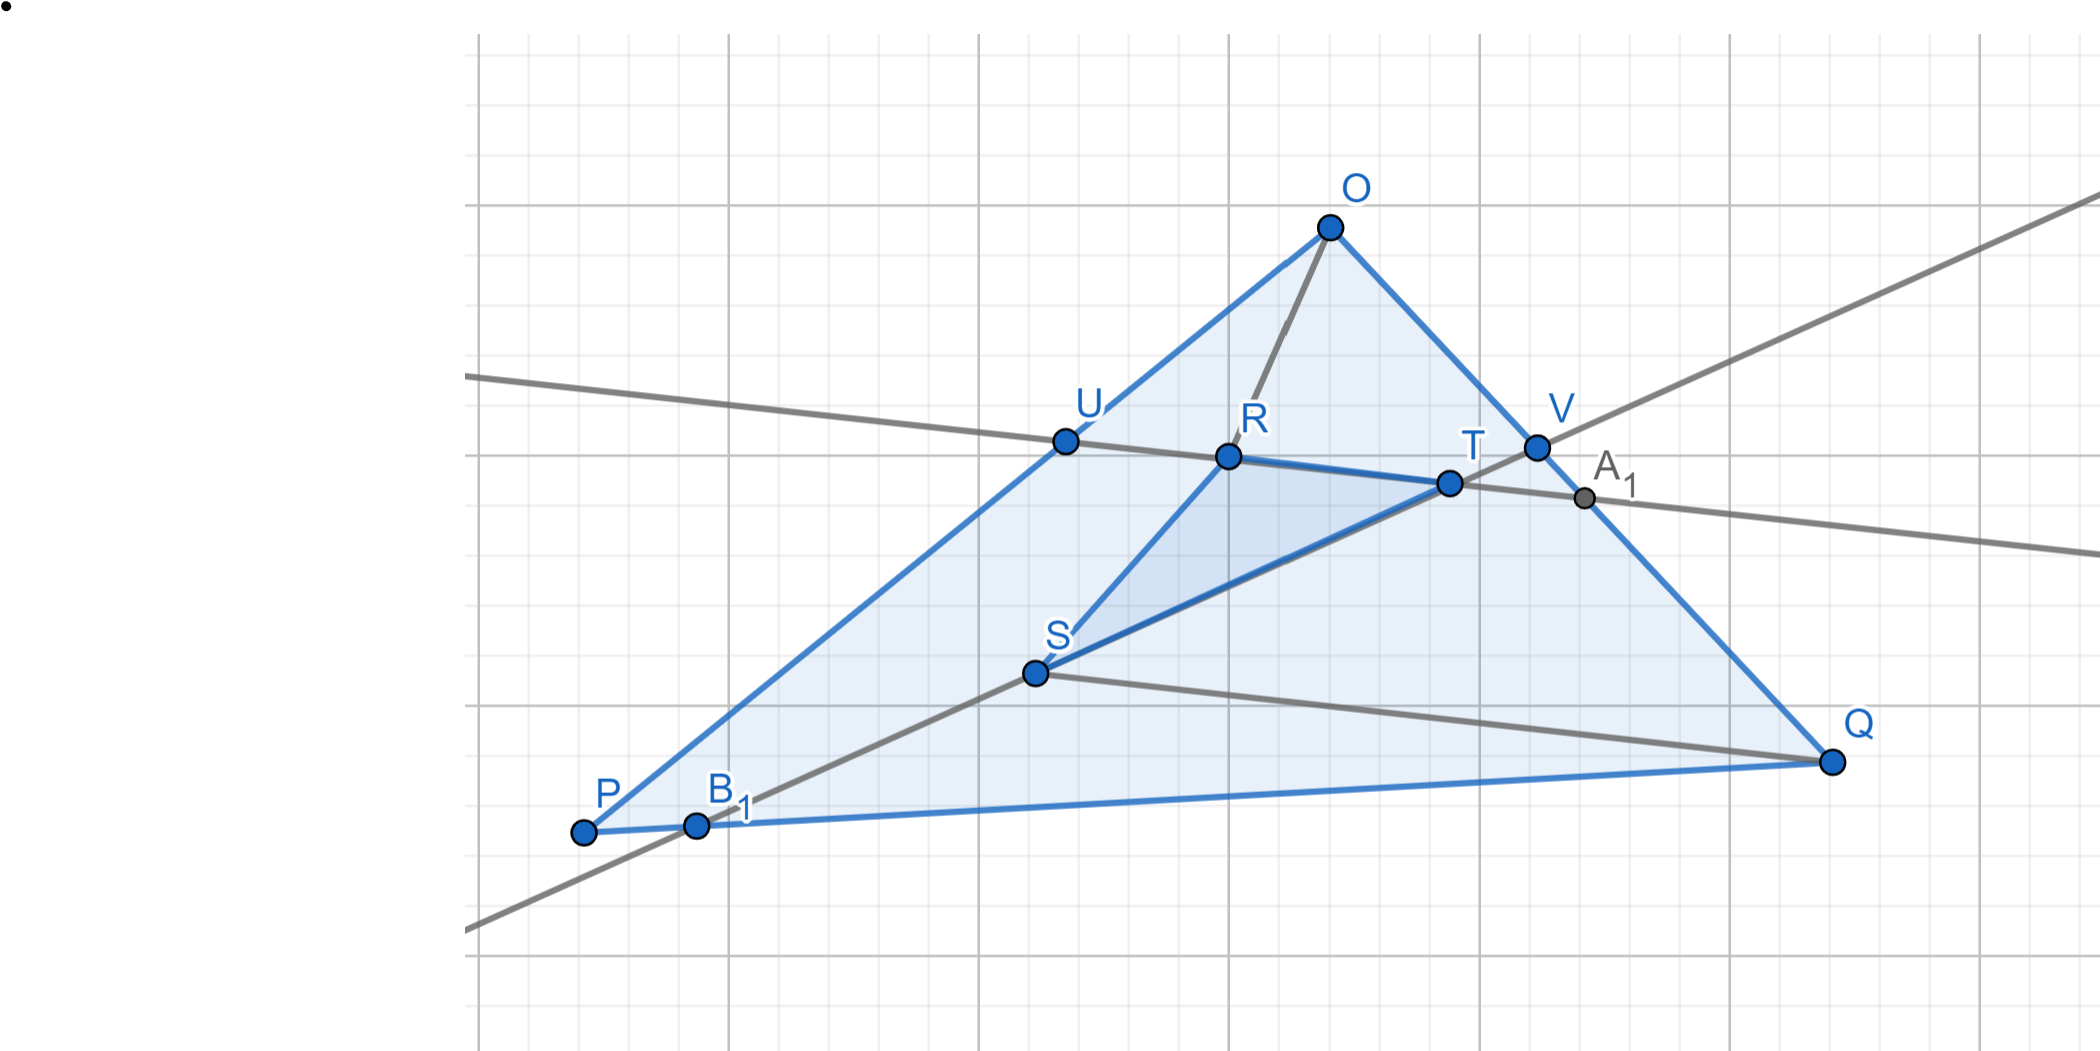
\includegraphics[scale=0.5]{triangularly_holy.png}
Now we can finally prove the theorem.


\begin{proof} 
For brevity and whimsy's sake, we shall call such a setup a \textbf{holy polygon}, and denote it $PH = P\setminus H \cup \bndry H$. We proceed by induction on the number of vertices in $PH$. Since the minimum number of vertices in a polygon is three, the minimum total number of vertices in a holy polygon is six. So for the base case, suppose that there are six total vertices. Then we have a triangle within a triangle. It is easy to see that a triangularly holy triangle can be triangulated. For select any vertex of the inner triangle, and any vertex of the outer triangle. Since a triangle is convex, there exists a line from the inner vertex to the outer one. Suppose it does not cross the boundary of the inner triangle. Then select another vertex. If not, it must cross the boundary at an edge of the inner triangle. Then any of the vertices of that edge can connect the the outer vertex.    \\

Now suppose that all holy polygons with less total number of vertices than $n$ are triangulizable. Since $P$ is itself a polygon, by a previous lemma there exists a diagonal $d$ from vertices in $P$. Because the holy polygon $PH$ is in general position, it cannot be the case that $H$ crosses either a vertex or edge of $H$. Hence there are two cases: either it does cross the boundary of $H$ (and it must cross the boundary of $H$ an even number of times), or it doesn't. 

\begin{enumerate}
\item Suppose it doesn't. Then $d$ divides $P$ into two polygons, $Q$ and $R$, such that $Q$ (without loss of generality) does not contain any of the points
of $H$ in its interior. Hence $Q$ is just a usual polygon, and by Theorem () of the textbook it can be triangulated. Moreover, by our induction hypothesis, since $RH$ is a holy polygon with at least one less vertices in total, $RH$ can be triangulated. Combining these two triangulations, we have a triangulation for $PH$.

\item Now suppose that $d$ does cross the boundary of $H$. Let the vertices of $d$ be $v_1$ and $v_2$. Notice that $d$ must cross the boundary a first and a last time (for it only crosses a finite number of times by the assumption of general position and the definition of a polygon). Moreover (again by our assumption of general position), these first and last crossings must occur at edges of $H$. Call these edges $e_1$ and $e_2$, and  call the corresponding points of intersection $x_1\in e_1$ and $x_2\in e_2$. Since $e_1$ and $e_2$ are edges, they have adjacent vertices. Let the vertices of the edge $e_1$ be $p_1$ and $p_2$, and the vertices of the edge $e_2$ be $q_1$ and $q_2$. Now chose some orientation for $H$, and without loss of generality, let $p_1$ be to the left of $p_2$, and $q_1$ be to the left of $q_2$ with respect to this orientation. Chose the orientation such that $p_2$ is to the left of $q_1$. Then since there are at least three vertices, $p_2$ is distinct from $q_2$. \\

Now construct the triangles $v_1x_1p_2$ and $v_2x_2q_2$. If neither of triangles contain points of $\bndry PH$, then $v_1p_2$ and $v_2q_2$ are disjoint diagonalizations of $PH$.\\

Suppose then that either one of them contains points of $\bndry PH$. Without loss of generality, suppose that $v_1x_1p_2$ contains at least one point of $\bndry PH$. Then it must cross at a vertex, and at a vertex closest to $v_1$. Then there are two cases: either that vetex belongs to $H$, or it belongs to $P$. If it belongs to $P$, we have a diagonal of $PH$ between between $P$ and $P$. If it belongs to $H$, we have a diagonal of $PH$ between $P$ and $H$. In the latter case, consider the other triangle, $v_1x_1p_2$. As with the first triangle, we have two cases: either it crosses $\bndry PH$ or it doesn't. If it doesn't, then we have a diagonal of $PH$ between $P$ and $H$ which is distinct from the first diagonal constructed. If it does, then we have two cases: either the closest vertex to $v_2$ belongs to $H$ or it belongs to $P$. In the first case, we have a diagonal between $P$ and $H$ which is distinct from the first. In the latter case, we have a diagonal between vertices of $P$ which stayes within the interior of $PH$. 

Hence there are really only two options: either we have a diagonal between $P$ and itself, in which case we can proceed as in case (1), or we have two disjoint diagonals between $P$ and $H$. This partitions the interior region of $PH$ into two polygons whose interiors are disjoint. These polygons can be triangulated. Combining these triangulations, we have a triangulation for $PH$. 

\end{enumerate}

Exhausting all of the cases, we see that $PH$ can be triangulated when it has $n$ vertices. Hence by induction a holy polygon with more than six vertices (and all holy polygons have more than six vertices) can be triangulated. 
\end{proof}

We can also extend this proof to polygons with any number of polygonal holes.

\begin{proposition} (Problem [])

Given a polygon $P$, with a polygonal hole $H$ with $h$ edges, such that both the polygon and the hole have a total of $n$ edges, each triangulation of the interior region contains exactly $n$ triangles. 

\end{proposition}

\begin{proof}
By the proof to one of the previous problems, we know that we triangulate the region between $P$ and $H$. Let $T$ be an arbitrary triangulation. Since triangulation will involve at least two disjoint diagonals, it follows that $T$ must divide $PH$ into two distinct polygons, call them $P_1$ and $P_2$. Moreover, $T$ triangulates $P_1$ and $P_2 $ when restricted.\\

 All of this has created no new vertices. Since we have created no new vertices, these polygons together must have all of the vertices of $PH$. They must also share exactly four of the vertices, for they are divided by two disjoint diagonals from $P$ to $H$, each of which contains two vertices. Let the number of vertices of $P_1$ be $n_1$ and similarly $n_2$ for $P_2$. Since together they contain all of the vertices of$PH$, sharing four of them, we have $n_1 + n_2 = n + 4$.\\
 
 Moreover, since $P_1$ and $P_2 $ are polygons, any triangulation of $P_1$ (including this one) must contain $n_1 - 2$ triangles, and similarly the number of triangles in the triangulation of $p_2$ is $n_2 - 2$
 
 Since the triangulations of $P_1$ and $P_2$ are the triangulations of $PH$ restricted to them, we have the following identity for the number of triangals in the triangulation of $PH$:
\[n_1 - 2 + n_2 -2 = (n_1 + n_2) - 4 = n + 4 -4 = n.\]

But $T$ was an arbitrary triangulation of $T$. Hence any triangulation of $PH$ must contain $n$ triangles.



\end{proof}


\newpage

\begin{proposition}
The polygon $P$, shown below, can't be divided by diagonals into quadrilaterals, though it has an even number of vertices

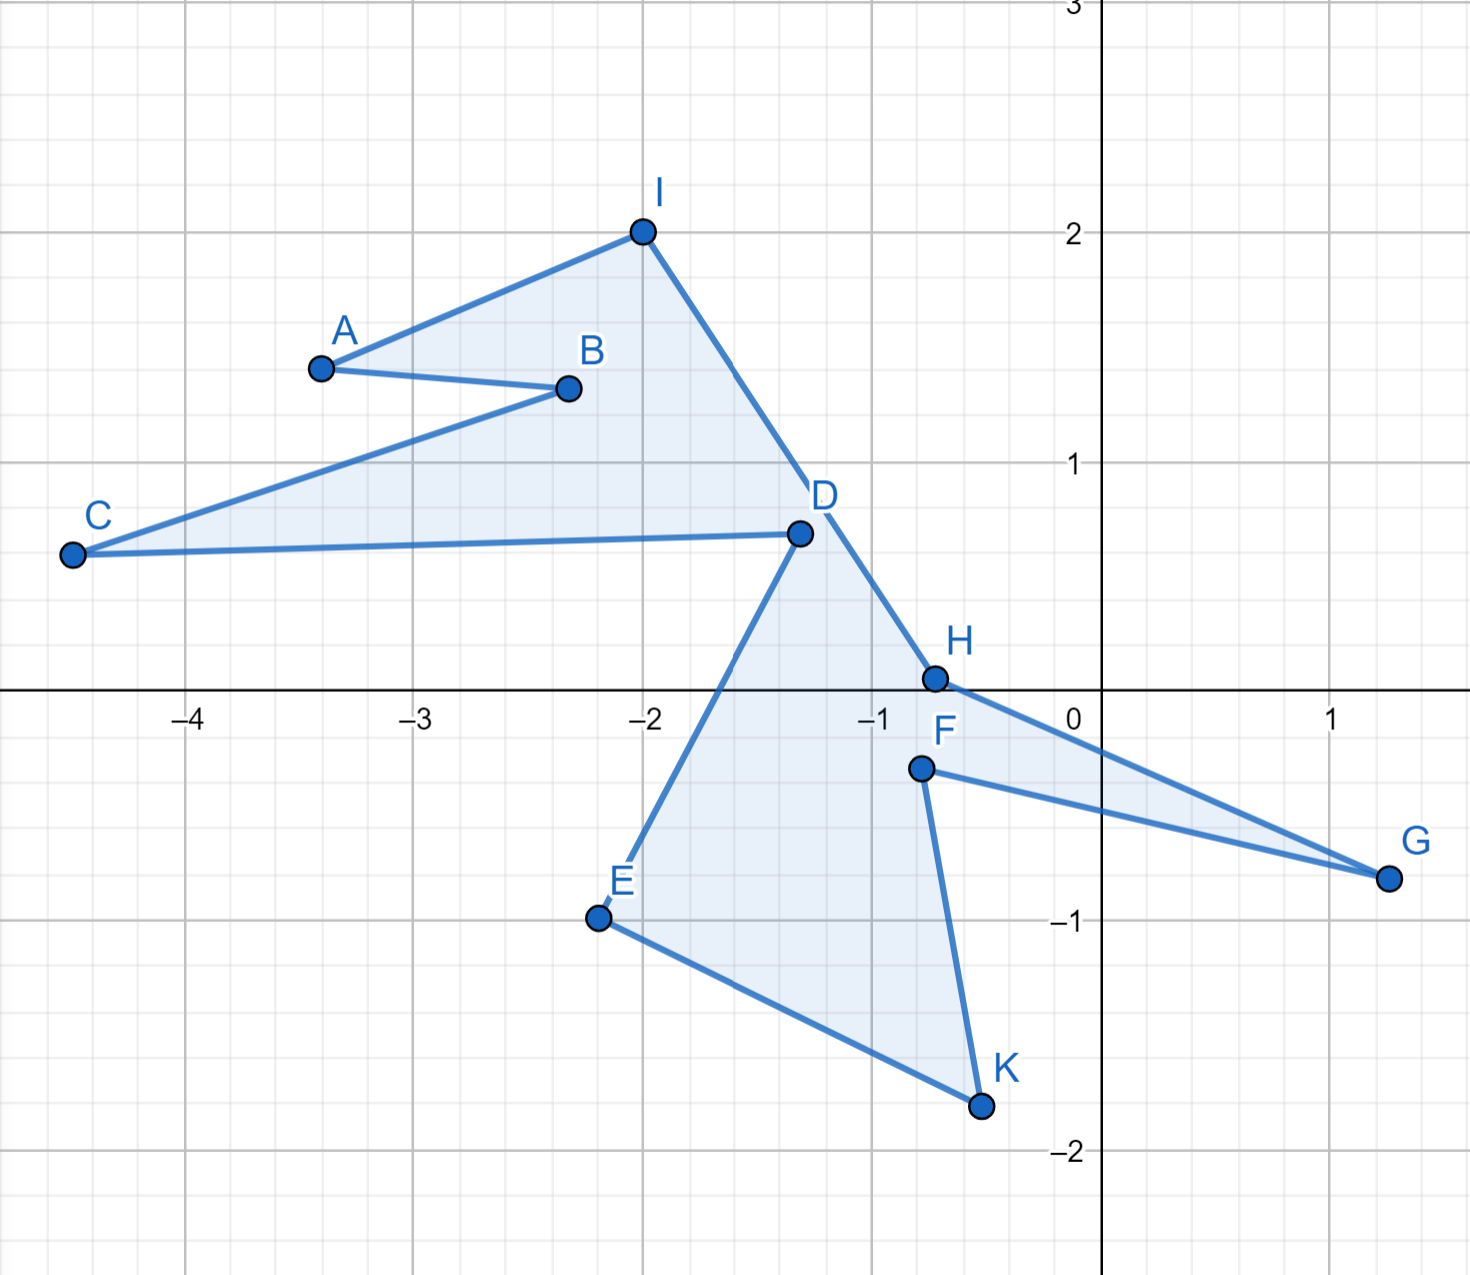
\includegraphics[scale=0.5]{cant_be_quaded.png}
\end{proposition}


\begin{proof}

Notice first of all that we must be able to turn the region containing $A$, $I$, and $D$ into a quadrilateral, for $A$ cannot connect by a diagonal to any vertices. Hence $B$ or $I$ must somehow connect to another vertex to close this region off. But if $I$ connects to $B$, we have a triangle. If $I$ connects to $D$, we have to also connect $B$ to $D$ in order to turn the region containing $A$, $I$ and $B$ into a quadrilateral. But this turns the region $C$, $B$, and $D$ into a triangle. Something similar happens if we first connect $B$ to $D.$
\end{proof}


\begin{proposition}
An orthogonal pyramid can be divided by diagonals into quadrilaterals. 
\end{proposition}

\begin{lemma}

Let $v$ be a vertex on an orthogonal pyramid, falling to one side, and let $u$ be a vertex on the other side. Suppose that $u$ is higher than or level to $v$. Suppose also that the diagonal $uv$ crosses the boundary. Then there must exist a reflex vertex on the same side of $v$ which is lower than $u$ but higher than $v$.
\end{lemma}

\begin{proof}

Notice that on an orthogonal pyramid, higher vertices are always closer to the center. Clearly $uv$ cannot cross the boundary on the side of $u$. Then it must cross on the side of $v$. Because it can't cross on one of the vertical edges, it must cross at a horizontal one. Clearly this horizontal edge must be higher than $v$. Moreover, other than the base and the roof, every edge of an orthogonal pyramid involves at least one reflex vertex. Because all reflex vertices are higher than or lower than the roof, it cannot be the case that $uv$ crosses through the roof or base. So it must cross through a horizontal vertex which contains a reflex vertex. Because that horizontal edge is higher than $v$, it must contain a reflex vertex which is higher than $v$ but lower than $u$. This is the vertex whose whose existence is purported by the lemma.

\end{proof}

\begin{remark}
I am still not satisfied, but I don't know what makes a proof satisfying. I need a philosopher, or a therapist (which are basically the same thing).
\end{remark}

\begin{proof} 

Draw a vertical line from the midpoint of the highest horizontal edge to the base. All of the vertices fall to the right or left this line. Let $v_1$ and $ u_1$ be the highest reflex vertices on the left and right respectively. Without loss of generality, suppose that $v_1$ has the minimum height of the two of them. Draw diagonals from $v_1$ to each of the vertices on the other side which higher than or lower than $v_1$. (By construction there is at least one of them).

Now let $p_1$ be the lowest vertex on the side of $u_1$ which has a diagonal drawn so far which connects it to $v_1$. Let $u_2$ be the vertex on the side of $u_1$ which is \textit{immediately} (note immediately) lower than $p_1$. (does it exist). Now let $v$ be a vertex on the side of $v$, which is lower than or level to $v_1$, and also higher than or level to $u$. Suppose by way of contradiction that the diagonal $u_2v$ cannot be drawn. Then by Lemma 1 there must exist a vertex $ u $ which is both higher than $u$ but lower than $v$. But since $v$ is lower than $v_1$, and since $u_1$ is the highest vertex which is lower than $v_1$, it follows that $u$ cannot exist. So the diagonal $u_2v$ must be able to be drawn. But $v$ was an arbitrary vertex on the side of $v_1$, and which is lower than or equal to $v_1$, and which is higher than or level with $u_2$. Therefore we can draw a diagonal from $u_2$ to any of the vertices on the side of $v_1$ which are lower than or equal to $v_1$, and which are level with or higher than $u_2$. Specifically, we can draw a diagonal from $u_2$ to every \textit{reflex} vertex $v$ which is lower than or level to $v_1$ and higher than or level to $u_2$. Moreover, because each of the $v$'s is lower than $v_1$, none of these diagonals cross the previously constructed ones. \\

Each of these diagonals divides the top region (all the way past $v_1$) into quadrilaterals. Now we let $v_2$ be the highest vertex on the side of $v_1$ and which does not have a diagonal connecting to it. Then we can repeat the same argument as with $u_2$ to construct diagonals, which will once again divide into quadrilaterals. \\

We now continue this process until we run out of either vertices on the left or the right. Without loss of generality, suppose we run out on the left. Let $v_i$ be the last vertex on the right from the iteration before it. Now select the bottom vertex on the left. Then we can draw a diagonal from this vertex to each of the vertices which are below or equal to $v_i$, using a similar argument as we did for the last few steps. This will divide the remaining bit of the pyramid into quadrilaterals. \\


\end{proof}

\begin{example}


 


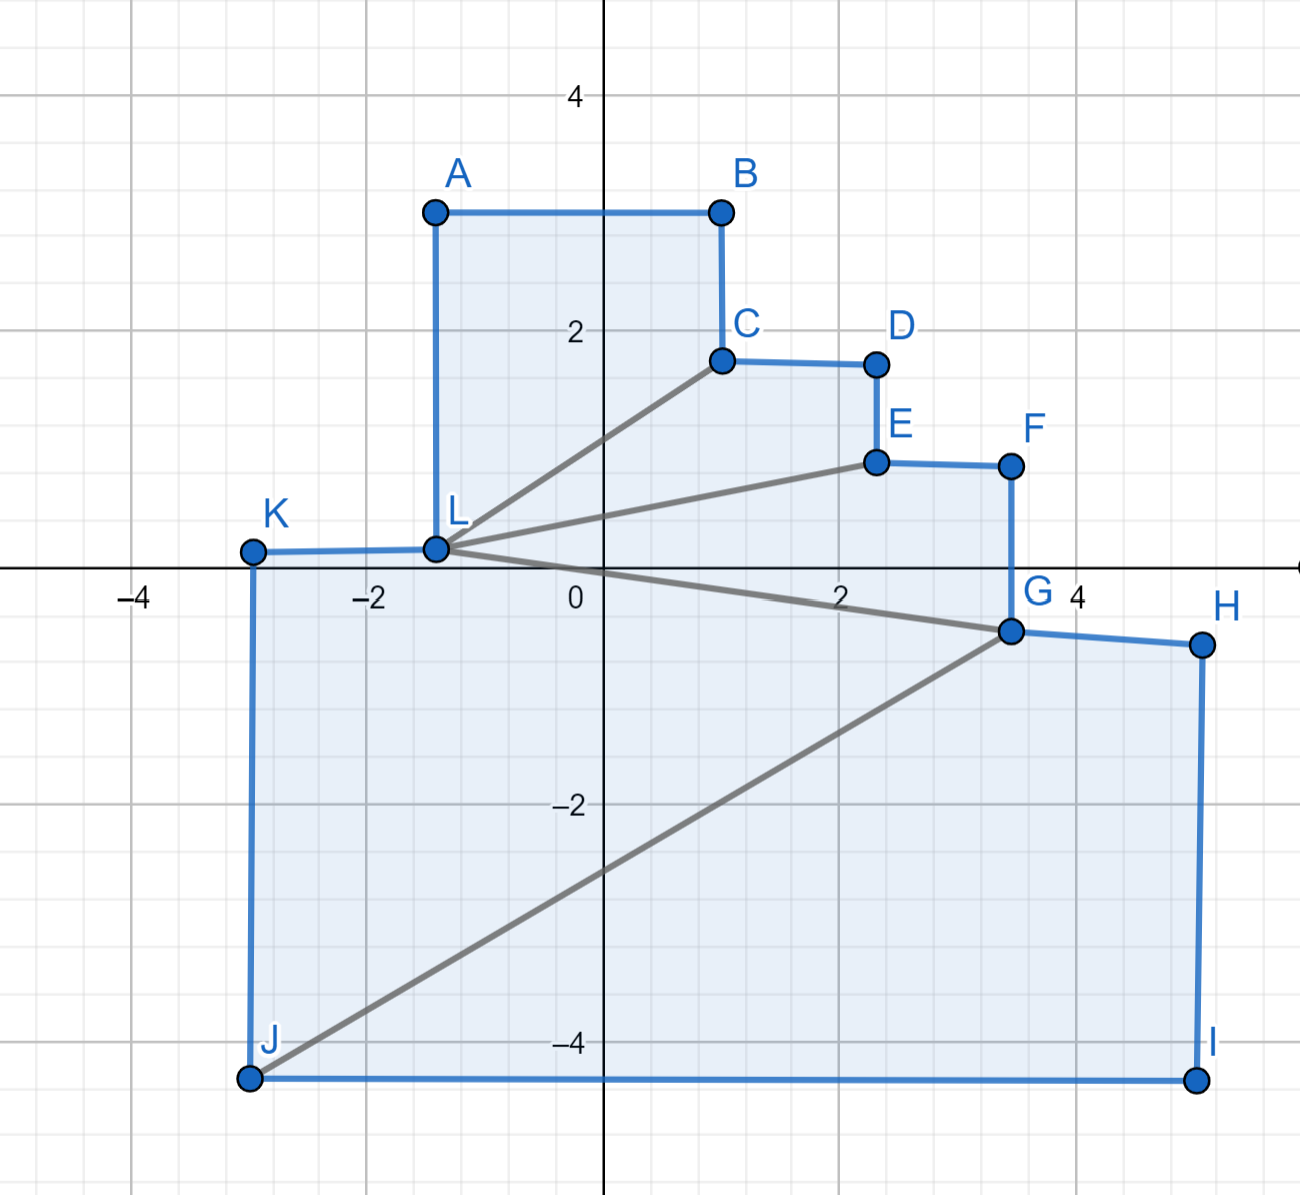
\includegraphics[scale=0.5]{orthogonal_pyramid_example.png}



In this example, we first select $L$. Since $C$ and $E$ are higher than $L$, we draw diagonals $ LC $ and $ LE $. This is all we can do, so we select the reflex vertex on the opposite side of $L$ which is immediately below $E$, which in this case is $G$. Since $L$ is above $G$, and equal to or lower than $L$, we draw the diagonal $LG$. This exhausts all of the reflex vertices, so we select the bottom vertex which is on the opposite side of $G$, namely $J$. Since $G$ is the only vertex on the opposite side of $J$ which is lower than or equal to $G$ (and higher than $J$ since $J$ is a bottom vertex), we only draw one more diagonal: $JG$. As you can see, this algorithm has succeeded in dividing the orthogonal pyramid into quadrilaterals. 
\end{example}

\begin{proposition}(1.16)
Consider any real valued function $f$ whose second derivative exists and is positive from $a$ to $b$, and such that $f(x) > 0 \forall x\in [a,b]$. Now chose some $c\in (a,b),$ and select $n-3$ real numbers $x_1, \dots, x_{n-3}\in [a,b]$. Now construct the polygon $ P = (0,c), (a, f(a)), (x_1, f(x_1)), \dots , (x_{n-3}, f(x_{n-3})), (b, f(b))$ with edges drawn cyclically. Then this polygon is a polygon with $n> 3$ vertices, and has a unique triangulation for all $n > 3$. 

\end{proposition}

\begin{proof}

Since, as we know from calculus, the region above a function with a positive second derivative is positive is convex. Call this region $R$. Also, $B = [a,b] \times \R$ is convex, hence the intersection of $R$ with $B$ is also convex; call this region $S$. This is the region of space above and including the curve carved out by $f$, and on the interval from $a$ to $b$. Now consider any $x_i$, $x_j$, where $i < j$ and the points $p_1 = (x_i, f(x_i),p_2 = (x_j, f(x_j)$ are not adjacent. Since $x_i,x_j\in [a,b]$, it follows that $p_1,p_2\in S$. \\

Now since $p_1$ and $p_2$ are not adjacent, there must exist some $q$ which is between $p_1$ and $p_2$, and $q$ must be of the form $(x_k, f(x_k))$ for $x_i < x_k < x_j$. Moreover, the point $v = (x_k, f(x_i) + f'(x_i)(x_k - x_i) )$ is between the points $p_1$ and $p_2$, which are oth members of $S$. Since $S$ is convex, it follows that $v\in S$. Hence $f(x_i) + f'(x_i)(x_k - x_i) \le f(x_k)$. But this means that the point $v$ is either equal to $q$, in which case $v \in \bndry P$, or else $v$ is exterior to $P$. In either case, $p_1p_2$ cannot be a diagonal of $P$. \\

$p_1$ and $p_2$ were arbitrary non-adjacent points of the form $(x_i, f(x_i)$. Since all diagonals connect non-adjacent points, it follows that no points of the form $(x_i, f(x_i)$ can be connected to each other by diagonals. But there must be a triangulation, which consists of diagonals, for $P$ is a polygon. So each of these diagonals are between of the form $(x_i, f(x_i)$. But since by construction of $P$, there is only one vertex, $p = (0,c) $, which is not of this form. It follows that all diagonals must connect to this point. Since all triangulations have the same number of diagonals (Theorem () of the textbook), it follows that only by connecting all points other than $p$ to $p$ can we form a triangulation of $P$. So there is only one triangulation for $P$.
\end{proof}


\begin{conjecture}

I conjecture that every polygon which has a unique triangulation can be rotated into one of this form.
\end{conjecture}



\end{document}
